\subsection{BME280}
\label{BME280}
{\begin{minipage}[b][6cm][t]{0.55\textwidth}
Der \textit{BME280} ist ein low powered digitaler Feuchtigkeits-, Luftdruck- und Temperatursensor von Bosch. Er ist in einem 2.5mm x 2.5mm x 0.93mm metal lid LGA Gehäuse verpackt und kann über die Interfaces I$^{2}$C und SPI kommunizieren. Durch seinen niedrigen Stromverbrauch, große operating range der drei Messgrößen und schnellen Ansprechzeit von etwa 1s eignet er sich für die solarbetriebene mobile Wetterstation besonders. \cite{Bosch2019}\\
\end{minipage}}
{\begin{minipage}[b][6cm][t]{0.44\textwidth}
\centering
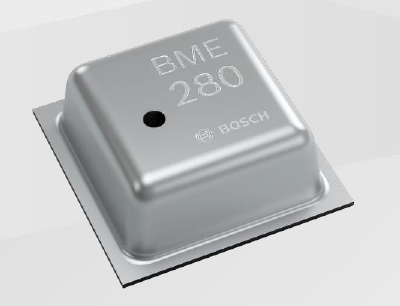
\includegraphics[width=0.9\textwidth]{graphics/bme280/bme280.PNG}
\captionof{figure}{BME280 \cite{Bosch2019}}
\label{fig:bme280}
%\vspace*{0.5cm}
%\centering
%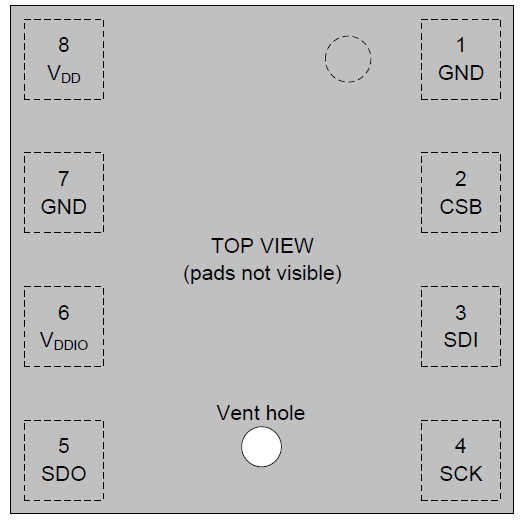
\includegraphics[width=0.9\textwidth]{graphics/bme280/bme280_pinout.PNG}
%\captionof{figure}{Pinout \cite{Bosch2019}}
%\label{fig:bme280_pinout}
\end{minipage}}

\begin{table}[h]
  \centering
  \caption{Elektrische Spezifikationen \cite{Bosch2019}}
    \begin{tabular}{lllll}
    \toprule
    \textbf{Parameter} & \textbf{Min.} & \textbf{Typ.} & \textbf{Max.} & \textbf{Einheit} \\
    \midrule
    Versorgungsspannung & 1.71  & 1.8   & 3.6   & V \\
    Stromverbrauch (sleep mode) &       & 0.1   & 0.3   & $\mu$A \\
    Stromverbrauch inaktiv (normal mode) &       & 0.2   & 0.5   & $\mu$A \\
    Stromverbrauch Feuchtigkeitsmessung &       & 340   &       & $\mu$A \\
    Stromverbrauch Luftdruckmessung &       & 714   &       & $\mu$A \\
    Stromverbrauch Temperaturmessung &       & 350   &       & $\mu$A \\
    \bottomrule
    \end{tabular}%
  \label{tab:elektrische_Spezifikationen}%
\end{table}%

Bei einer Messfrequenz von 1Hz für die drei Messgrößen verbraucht der BME280 somit laut Datenblatt nur \textbf{3.6$\mu$A}. \cite[S. 2]{Bosch2019}

\subsubsection*{Feuchtigkeitsmessung}
In der Tabelle \ref{tab:spez_feuchtigkeit} sind die wichtigsten Parameter zur Feuchtigkeitsmessung aufgelistet. Zu vermerken ist, dass die digitalen Werte des BME280 zur Feuchtigkeitsmessung relativ sind und deshalb prozentual angegeben werden. \\
\begin{table}[htbp]
  \centering
  \caption{Sezifikationen der Feuchtigkeitsmessung \cite{Bosch2019}}
    \begin{tabular}{lllll}
    \toprule
     \textbf{Parameter} & \textbf{Min.} & \textbf{Typ.} & \textbf{Max.} & \textbf{Einheit} \\
    \midrule
    Operating range & -40   & 25    & 85    & $^{o}$C \\
          & 0     &       & 100   & \% \\
    Absolute Genauigkeitstoleranz &       & $\pm$3 &       & \% \\
    Hysterese &       & $\pm$1 &       & \% \\
    Auflösung &       & 0.008 &       & \% \\
    Langzeitstabilität &       & 0.5   &       & \% pro Jahr \\
    \bottomrule
    \end{tabular}%
  \label{tab:spez_feuchtigkeit}%
\end{table}%

\newpage

\subsubsection*{Luftdruckmessung}
Die Genauigkeit der Luftdruckmessung ist an einen Temperaturbereich gebunden. Bei niedrigeren Temperaturen (<0$^{o}$C) weist der Sensor eine höhere Unsicherheit auf als bei Temperaturen von 0 bis 65 $^{o}$C (siehe Tabelle \ref{tab:spez_druck}). \\
\begin{table}[htbp]
  \centering
  \caption{Sezifikationen der Luftdruckmessung \cite{Bosch2019}}
    \begin{tabular}{llllll}
    \toprule
    \textbf{Parameter} & \multicolumn{1}{l}{\textbf{Temperaturbereich}} & \multicolumn{1}{l}{\textbf{Min.}} & \textbf{Typ. } & \multicolumn{1}{l}{\textbf{Max.}} & \textbf{Einheit} \\
    \midrule
    Operating range &       & \multicolumn{1}{l}{-40} & 25    & \multicolumn{1}{l}{85} & $^{o}$C \\
          &       & 300   &       & 1100  & hPa \\
    Absolute Genauigkeit & \multicolumn{1}{c}{-20 bis 0 $^{o}$C} &       & $\pm$1.7 &       & hPa \\
          & \multicolumn{1}{c}{0 bis 65 $^{o}$C} &       & $\pm$1  &       & hPa \\
    Auflösung &       &       & \multicolumn{1}{r}{0.18} &       & hPa \\
    Langzeitstabilität &       &       & $\pm$1  &       & hPa pro Jahr \\
    \bottomrule
    \end{tabular}%
  \label{tab:spez_druck}%
\end{table}%

\subsubsection*{Temperaturmessung}
Die Wetterstation wird hauptsächlich in einem Temperaturbereich von 0 bis 65 $^{o}$C betrieben, wodurch vom Sensor eine Unsicherheit von max. $\pm$1 $^{o}$C erreicht werden kann. \\
\begin{table}[htbp]
  \centering
  \caption{Sezifikationen der Temperaturmessung \cite{Bosch2019}}
    \begin{tabular}{llllll}
    \toprule
    \textbf{Parameter} & \multicolumn{1}{l}{\textbf{Temperaturbereich}} & \multicolumn{1}{l}{\textbf{Min.}} & \textbf{Typ. } & \multicolumn{1}{l}{\textbf{Max.}} & \textbf{Einheit} \\
    \midrule
    Operating range &       & \multicolumn{1}{l}{-40} & 25    & \multicolumn{1}{l}{85} & $^{o}$C \\
    Absolute Genauigkeit & \multicolumn{1}{c}{25 C} &       & $\pm$0.5 &       & $^{o}$C \\
          & \multicolumn{1}{c}{0 bis 65 C} &       & $\pm$1  &       & $^{o}$C \\
          & \multicolumn{1}{c}{-20 bis 0 C} &       & $\pm$1.25 &       & $^{o}$C \\
          & \multicolumn{1}{c}{-40 bis -20 C} &       & $\pm$1.5 &       & $^{o}$C \\
    Auflösung  &       &       & 0.01  &       & $^{o}$C \\
    \bottomrule
    \end{tabular}%
  \label{tab:spez_temp}%
\end{table}%

\subsubsection*{Implementation in die Firmware}
Um den BME280 vom Microcontroller aus ansteuern zu können, wurden zwei bereits existierende Librarys von Adafruit verwendet:
\begin{itemize}
\item Adafruit BME280 Library
\item Adafruit Unified Sensors
\end{itemize}
Anschließend konnten die Headerfiles <Adafruit\_Sensor.h> und <Adafruit\_BME280.h> inkludiert werden und der Sensor über das I$^{2}$C Interface mit den folgenden Funktionen abgefragt werden:\\
\begin{itemize}
\item \textcolor{blue}{float} \textcolor{orange}{readTemperature}()
\item \textcolor{blue}{float} \textcolor{orange}{readHumidity}()
\item \textcolor{blue}{float} \textcolor{orange}{readPressure}()
\end{itemize}